\documentclass[UTF8,9pt]{ctexbeamer}

% "流体我闻" style adaptation:
% 4:3 default Beamer, compact white pages, formula-first explanations,
% colored formula annotations, dense but stable minipage/tabular layouts.

\usepackage[utf8]{inputenc}
\usepackage{amsmath}
\usepackage{amsfonts}
\usepackage{amssymb}
\usepackage{graphicx}
\usepackage{epstopdf,epsfig}
\usepackage{tabularx}
\usepackage{booktabs}
\usepackage{xcolor}
\usepackage{soul}
\usepackage{multicol}
\usefonttheme{professionalfonts}
\usepackage[absolute,overlay]{textpos}
\usepackage{mathtools,physics,cancel,array,ulem,longtable,ragged2e,mathrsfs,extarrows,bm}
\usepackage{pifont,bbding}
\usepackage{tikz}
\usetikzlibrary{arrows.meta,positioning,calc,decorations.pathreplacing}

\usetheme{default}
\usecolortheme{default}
\useinnertheme{default}
\setbeamercolor{structure}{fg=blue!70!black}
\setbeamercolor{frametitle}{fg=blue!70!black}
\setbeamercolor{title}{fg=blue!70!black}
\setbeamercolor{subtitle}{fg=blue!70!black}
\setbeamercolor{alerted text}{fg=red}
\setbeamerfont{title}{size=\large,series=\mdseries}
\setbeamerfont{subtitle}{size=\large,series=\mdseries}
\setbeamerfont{frametitle}{size=\large,series=\mdseries}
\setbeamerfont{section in toc}{size=\small,series=\mdseries}
\setbeamerfont{subsection in toc}{size=\footnotesize,series=\mdseries}
\setbeamersize{text margin left=1.2em,text margin right=1.2em}

\hypersetup{colorlinks=false,pdftitle={Fluid Mechanics: Continuum}}

\renewcommand{\dd}{\,\mathrm{d}}
\newcommand{\Dt}{\mathrm{D}}
\newcommand{\uvec}{\bm{u}}
\newcommand{\xvec}{\bm{x}}
\renewcommand{\grad}{\bm{\nabla}}
\newcommand{\Kn}{\mathrm{Kn}}
\newcommand{\Ma}{\mathrm{Ma}}
\newcommand{\cyan}[1]{{\color{cyan}#1}}
\newcommand{\teal}[1]{{\color{teal}#1}}
\newcommand{\olive}[1]{{\color{olive}#1}}
\newcommand{\purple}[1]{{\color{purple}#1}}
\newcommand{\red}[1]{{\color{red}#1}}
\newcommand{\graytxt}[1]{{\color{gray}#1}}
\newcommand{\btri}{\textcolor{blue!75!black}{$\blacktriangleright$}}
\newcommand{\toclink}[2]{\hyperlink{#1}{#2}}
\newcommand{\rev}{\delta\mathscr{V}}
\newcommand{\vol}{\mathscr{V}}

\author{重庆大学土木工程学院}
\title{Fluid Mechanics:\\[3pt]Continuum}
\subtitle{连续性假设与流体基本描述}
\date{2026 年秋季学期}

\begin{document}

\begin{frame}
\titlepage
\end{frame}

\begin{frame}{Contents}
\footnotesize
\begin{multicols}{2}
\toclink{molecule}{\textcolor{blue!70!black}{continuum assumption}}

\hspace{.25cm}\toclink{molecule}{molecule vs. field}

\hspace{.25cm}\toclink{rev}{representative volume}

\hspace{.25cm}\toclink{kn}{Knudsen number}

\vspace{.24cm}
\toclink{density}{\textcolor{blue!70!black}{fluid variables}}

\hspace{.25cm}\toclink{density}{density}

\hspace{.25cm}\toclink{velocity}{velocity}

\hspace{.25cm}\toclink{pressure}{pressure}

\hspace{.25cm}\toclink{viscosity}{viscosity}

\vspace{.24cm}
\toclink{material}{\textcolor{blue!70!black}{descriptions and equations}}

\hspace{.25cm}\toclink{material}{material derivative}

\hspace{.25cm}\toclink{incompressible}{incompressibility}

\hspace{.25cm}\toclink{noslip}{boundary conditions}

\vspace{.24cm}
\toclink{failure}{\textcolor{blue!70!black}{limits and practice}}

\hspace{.25cm}\toclink{failure}{continuum failure}

\hspace{.25cm}\toclink{practice}{estimation}
\end{multicols}
\end{frame}

\section{continuum assumption}
\subsection{molecule vs. field}

\begin{frame}[label=molecule]{molecules $\Longrightarrow$ continuum field}
\[
\boxed{\quad
\rho=\rho(\xvec,t),\qquad
\uvec=\uvec(\xvec,t),\qquad
p=p(\xvec,t)
\quad}
\]

\vspace{.16cm}
\begin{tabular}{m{.47\textwidth}m{.47\textwidth}}
\small
\btri\ microscopic:
\[
\text{molecules}\quad\graytxt{\longrightarrow}\quad\red{\text{fluctuation}}
\]
\btri\ local average:
\[
\Delta\vol \longrightarrow \cyan{\rev}
\]
\btri\ macroscopic:
\[
\rho,\ \uvec,\ p\quad\graytxt{\longrightarrow}\quad\olive{\text{smooth fields}}
\]
&
\centering
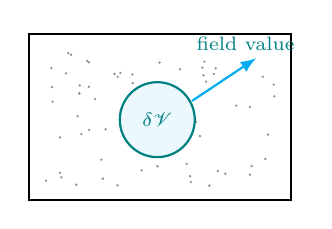
\begin{tikzpicture}[scale=.68]
  \draw[thick] (0,0) rectangle (4.9,3.1);
  \foreach \i in {1,...,70}{
    \pgfmathsetmacro{\x}{.25+4.35*rnd}
    \pgfmathsetmacro{\y}{.25+2.55*rnd}
    \fill[black!45] (\x,\y) circle (.024);
  }
  \draw[thick,teal,fill=cyan!8] (2.4,1.5) circle (.7);
  \node[teal] at (2.4,1.5) {\scriptsize $\rev$};
  \draw[-{Latex[length=2mm]},thick,cyan] (3.05,1.85) -- (4.25,2.65);
  \node[teal] at (4.05,2.92) {\scriptsize field value};
\end{tikzpicture}
\end{tabular}

\vspace{.14cm}
\olive{\scriptsize key: average over enough molecules, but keep the volume small compared with the flow scale.}
\end{frame}

\subsection{representative volume}

\begin{frame}[label=rev]{fluid particle: not a molecule, not the whole flow}
\[
\text{molecular scale}
\quad \ll \quad
\alert{\text{fluid particle scale}}
\quad \ll \quad
\text{flow length scale}
\]

\vspace{.18cm}
\begin{tabular}{m{.47\textwidth}m{.47\textwidth}}
\small
\btri\ many molecules: stable average

\vspace{.12cm}
\btri\ small volume: local point

\vspace{.12cm}
\btri\ moves with local variables
&
\centering
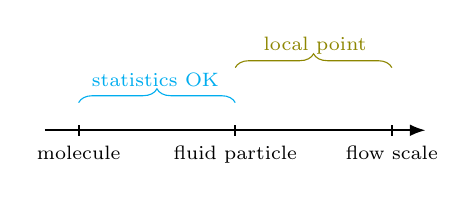
\begin{tikzpicture}[scale=.78]
  \draw[-{Latex[length=2mm]},thick] (0,0) -- (6.2,0);
  \foreach \x/\lab in {.55/molecule,3.1/fluid particle,5.65/flow scale}{
    \draw[thick] (\x,-.09) -- (\x,.09);
    \node[below] at (\x,-.1) {\scriptsize \lab};
  }
  \draw[decorate,decoration={brace,amplitude=5pt},cyan] (.55,.45) -- (3.1,.45);
  \node[cyan] at (1.8,.82) {\scriptsize statistics OK};
  \draw[decorate,decoration={brace,amplitude=5pt},olive] (3.1,1.02) -- (5.65,1.02);
  \node[olive] at (4.4,1.38) {\scriptsize local point};
\end{tikzpicture}
\end{tabular}

\vspace{.2cm}
\[
\rho(\xvec,t)=
\lim_{\Delta \vol\rightarrow\rev}
\frac{\Delta m}{\Delta \vol},
\qquad
\red{\rev \neq 0\ \text{physically}}
\]
\end{frame}

\subsection{Knudsen number}

\begin{frame}[label=kn]{$\Kn=\lambda/L$: criterion for continuum}
\[
\boxed{\displaystyle
\Kn=\frac{\cyan{\lambda}}{\purple{L}}
}
\qquad
\begin{array}{ll}
\cyan{\lambda}: & \text{molecular mean free path}\\[2pt]
\purple{L}: & \text{flow/geometric length scale}
\end{array}
\]

\vspace{.15cm}
\begin{center}
\small
\begin{tabular}{lll}
\toprule
range & description & model idea \\
\midrule
$\Kn<10^{-3}$ & continuum & Navier--Stokes usually OK \\
$10^{-3}\sim10^{-1}$ & slip/transition & boundary condition matters \\
$\Kn>10^{-1}$ & rarefied & continuum may fail \\
\bottomrule
\end{tabular}
\end{center}

\vspace{.16cm}
\small
\btri\ continuum is not ``molecules disappear''; it is a controlled averaging.
\end{frame}

\begin{frame}{civil engineering scales: usually safe}
\begin{tabular}{m{.44\textwidth}m{.50\textwidth}}
\small
\btri\ air at standard condition:
\[
\lambda\sim 10^{-8}\ \mathrm{m}
\]
\btri\ pipes, buildings, rivers:
\[
L\gg\lambda
\]
\btri\ micro gas flow: check $\Kn$
&
\centering
\small
\begin{tabular}{lll}
\toprule
case & $L$ & $\Kn$ \\
\midrule
building wind & $10\ \mathrm{m}$ & $\sim 10^{-8}$\\
ventilation duct & $0.1\ \mathrm{m}$ & $\sim 10^{-6}$\\
micro-channel gas & $1\ \mu\mathrm{m}$ & $\sim 10^{-2}$\\
\bottomrule
\end{tabular}
\end{tabular}

\vspace{.32cm}
\[
\underbrace{\lambda \ll L}_{\text{\cyan{scale separation}}}
\quad \Longrightarrow \quad
\underbrace{\rho,\ \uvec,\ p\ \text{are fields}}_{\text{\olive{continuum model}}}
\]
\end{frame}

\section{fluid variables}
\subsection{density}

\begin{frame}[label=density]{density: local average}
\[
\rho(\xvec,t)=
\lim_{\Delta \vol\rightarrow\rev}
\frac{\Delta m}{\Delta \vol}
\qquad
\begin{array}{rcl}
\Delta \vol \ \text{too small} &\Rightarrow& \red{\text{fluctuation}}\\
\Delta \vol \ \text{too large} &\Rightarrow& \red{\text{smearing}}\\
\Delta \vol \rightarrow \rev &\Rightarrow& \cyan{\text{stable local value}}
\end{array}
\]

\vspace{.1cm}
\begin{center}
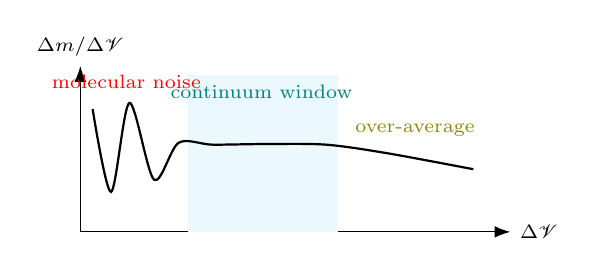
\begin{tikzpicture}[x=1cm,y=1cm,scale=.78]
  \draw[-{Latex[length=2mm]}] (0,0) -- (7,0) node[right] {\scriptsize $\Delta \vol$};
  \draw[-{Latex[length=2mm]}] (0,0) -- (0,2.7) node[above] {\scriptsize $\Delta m/\Delta\vol$};
  \draw[fill=cyan!8,draw=none] (1.75,0) rectangle (4.2,2.55);
  \draw[thick,smooth] plot coordinates{(.2,2.0)(.5,.65)(.8,2.1)(1.2,.85)(1.6,1.45)(2.15,1.42)(3.0,1.43)(4.0,1.42)(5.0,1.28)(6.4,1.02)};
  \node[teal] at (2.95,2.28) {\scriptsize continuum window};
  \node[red] at (.75,2.45) {\scriptsize molecular noise};
  \node[olive] at (5.45,1.65) {\scriptsize over-average};
\end{tikzpicture}
\end{center}
\end{frame}

\subsection{velocity}

\begin{frame}[label=velocity]{velocity field: components and local value}
\[
\uvec(\xvec,t)
=u(\xvec,t)\vec e_1+v(\xvec,t)\vec e_2+w(\xvec,t)\vec e_3
\]

\begin{tabular}{m{.43\textwidth}m{.51\textwidth}}
\small
\btri\ vector value at every point:
\[
\xvec=(x_1,x_2,x_3)
\]
\btri\ acceleration is not only $\partial\uvec/\partial t$
\[
\frac{\Dt\uvec}{\Dt t}
=\frac{\partial\uvec}{\partial t}
+(\uvec\cdot\grad)\uvec
\]
&
\centering
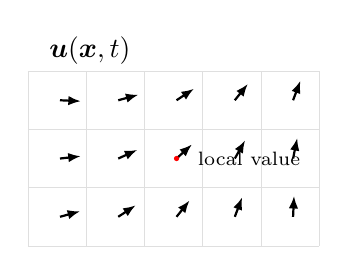
\begin{tikzpicture}[scale=.74]
  \draw[step=1,gray!25,very thin] (0,0) grid (5,3);
  \foreach \x in {.55,1.55,2.55,3.55,4.55}{
    \foreach \y in {.5,1.5,2.5}{
      \pgfmathsetmacro{\ang}{10+18*\x-9*\y}
      \draw[-{Latex[length=1.6mm]},thick] (\x,\y) -- ++(\ang:.36);
    }
  }
  \node[anchor=west] at (.2,3.35) {$\uvec(\xvec,t)$};
  \fill[red] (2.55,1.5) circle (.045);
  \node[anchor=west] at (2.75,1.5) {\scriptsize local value};
\end{tikzpicture}
\end{tabular}
\end{frame}

\begin{frame}{Eulerian vs. Lagrangian}
\[
\begin{array}{rclcl}
\text{\alert{Eulerian}} &:&
\uvec &=& \uvec(\xvec,t)
\qquad \text{\small fixed point in space}\\[4pt]
\text{\cyan{Lagrangian}} &:&
\xvec &=& \xvec(\xvec_0,t)
\qquad \text{\small follow a fluid particle}
\end{array}
\]

\vspace{.16cm}
\begin{tabular}{m{.45\textwidth}m{.45\textwidth}}
\textcolor{red}{Eulerian}
\begin{itemize}
\item control equations
\item boundary conditions
\item CFD / PIV / probes
\end{itemize}
&
\textcolor{cyan}{Lagrangian}
\begin{itemize}
\item particle trajectory
\item material derivative
\item tracer particles
\end{itemize}
\end{tabular}

\vspace{.05cm}
\[
\boxed{\displaystyle
\frac{\Dt(\cdot)}{\Dt t}
=
\underbrace{\frac{\partial(\cdot)}{\partial t}}_{\cyan{\text{local}}}
+
\underbrace{\uvec\cdot\grad(\cdot)}_{\olive{\text{convective}}}}
\]
\end{frame}

\subsection{pressure}

\begin{frame}[label=pressure]{pressure: normal force per unit area}
\[
p=\lim_{\Delta A\rightarrow 0}
\frac{\Delta F_n}{\Delta A}
\qquad
\red{\text{force}}\ \perp\ \cyan{\text{surface}}
\]

\begin{tabular}{m{.45\textwidth}m{.48\textwidth}}
\small
\btri\ hydrostatics: same pressure in all directions

\vspace{.13cm}
\btri\ moving flow: pressure + viscous stresses

\vspace{.13cm}
\btri\ wind load, pipe flow, outlet jet
&
\centering
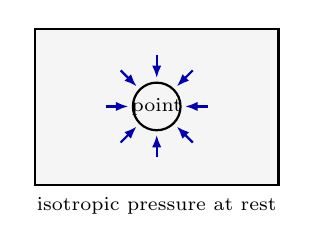
\begin{tikzpicture}[scale=.72]
  \draw[thick,fill=gray!8] (0,0) rectangle (4.3,2.75);
  \draw[thick] (2.15,1.38) circle (.42);
  \foreach \a in {0,45,...,315}{
    \draw[-{Latex[length=1.6mm]},thick,blue!70!black] ($(2.15,1.38)+(\a:.9)$) -- ($(2.15,1.38)+(\a:.5)$);
  }
  \node at (2.15,1.38) {\scriptsize point};
  \node at (2.15,-.38) {\scriptsize isotropic pressure at rest};
\end{tikzpicture}
\end{tabular}
\end{frame}

\subsection{viscosity}

\begin{frame}[label=viscosity]{viscosity: velocity gradient produces shear}
\[
\tau=\mu\frac{\dd u}{\dd y}
\qquad
\begin{array}{rcl}
\mu &:& \text{dynamic viscosity}\\[2pt]
\dd u/\dd y &:& \text{shear rate}\\[2pt]
\tau &:& \text{viscous shear stress}
\end{array}
\]

\begin{tabular}{m{.43\textwidth}m{.50\textwidth}}
\small
\btri\ no velocity gradient: no Newtonian shear

\vspace{.13cm}
\btri\ viscosity creates boundary layers

\vspace{.13cm}
\btri\ pipe friction and wake dissipation
&
\centering
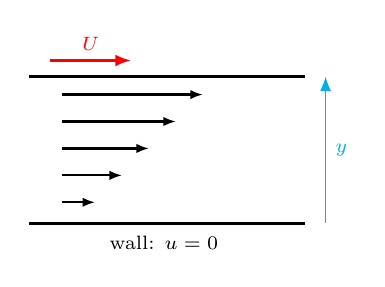
\begin{tikzpicture}[scale=.76]
  \draw[very thick] (0,0) -- (4.6,0);
  \draw[very thick] (0,2.45) -- (4.6,2.45);
  \draw[-{Latex[length=2mm]},thick,red] (.35,2.72) -- (1.7,2.72) node[midway,above] {\scriptsize $U$};
  \foreach \y/\len in {.35/.55,.8/1.0,1.25/1.45,1.7/1.9,2.15/2.35}{
    \draw[-{Latex[length=1.6mm]},thick] (.55,\y) -- ++(\len,0);
  }
  \draw[-{Latex[length=1.8mm]},cyan] (4.95,0) -- (4.95,2.45) node[midway,right] {\scriptsize $y$};
  \node at (2.25,-.33) {\scriptsize wall: $u=0$};
\end{tikzpicture}
\end{tabular}
\end{frame}

\section{descriptions and equations}
\subsection{material derivative}

\begin{frame}[label=material]{material derivative}
\[
\frac{\Dt \phi}{\Dt t}
=
\underbrace{\frac{\partial \phi}{\partial t}}_{\cyan{\text{unsteady at fixed point}}}
+
\underbrace{\uvec\cdot\grad\phi}_{\olive{\text{change due to motion}}}
\]

\vspace{.1cm}
\[
\text{for velocity:}\qquad
\frac{\Dt \uvec}{\Dt t}
=
\frac{\partial \uvec}{\partial t}
+u\frac{\partial\uvec}{\partial x}
+v\frac{\partial\uvec}{\partial y}
+w\frac{\partial\uvec}{\partial z}
\]

\vspace{.12cm}
\small
\btri\ this is the bridge between Lagrangian thinking and Eulerian equations

\vspace{.1cm}
\btri\ the nonlinear term appears because a particle moves through spatial gradients
\end{frame}

\subsection{incompressibility}

\begin{frame}[label=incompressible]{incompressible: not ``pressure cannot change''}
\[
\text{incompressible}
\quad \Longleftrightarrow \quad
\frac{\Dt \rho}{\Dt t}=0
\]

\vspace{.08cm}
\[
\frac{\Dt \rho}{\Dt t}
=
\frac{\partial \rho}{\partial t}
+\uvec\cdot\grad\rho,
\qquad
\text{mass conservation gives}
\qquad
\boxed{\grad\cdot\uvec=0}
\]

\vspace{.18cm}
\small
\btri\ liquids: often incompressible

\vspace{.11cm}
\btri\ low-speed gases: often incompressible when $\Ma<0.3$

\vspace{.11cm}
\btri\ pressure still varies; it enforces the velocity constraint
\end{frame}

\subsection{boundary conditions}

\begin{frame}[label=noslip]{boundary condition: no slip}
\[
\boxed{\uvec_{\text{fluid at wall}}=\uvec_{\text{wall}}}
\]

\vspace{.12cm}
\begin{tabular}{m{.43\textwidth}m{.50\textwidth}}
\small
\btri\ stationary wall:
\[
\uvec=0
\]
\btri\ moving wall:
\[
\uvec=\uvec_{\mathrm{wall}}
\]
\btri\ may fail for rarefied / micro-scale gas flows
&
\centering
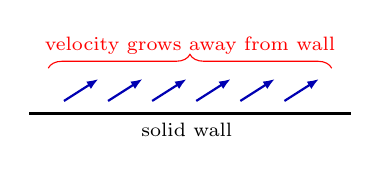
\begin{tikzpicture}[scale=.8]
  \draw[very thick] (0,0) -- (5.1,0);
  \foreach \x in {.55,1.25,1.95,2.65,3.35,4.05}{
    \draw[-{Latex[length=1.5mm]},thick,blue!70!black] (\x,.2) -- ++(.55,.35);
  }
  \node[below] at (2.5,0) {\scriptsize solid wall};
  \draw[red,decorate,decoration={brace,amplitude=5pt}] (.3,.72) -- (4.8,.72);
  \node[red] at (2.55,1.08) {\scriptsize velocity grows away from wall};
\end{tikzpicture}
\end{tabular}
\end{frame}

\section{limits and practice}
\subsection{continuum failure}

\begin{frame}[label=failure]{when continuum fails}
\begin{tabular}{m{.47\textwidth}m{.46\textwidth}}
\small
\btri\ high-altitude rarefied gas

\vspace{.14cm}
\btri\ micro / nano channels

\vspace{.14cm}
\btri\ strong non-equilibrium near shocks

\vspace{.14cm}
\btri\ molecular-scale evaporation / condensation
&
\[
\Kn=\frac{\lambda}{L}
\quad
\begin{cases}
\ll 1, & \text{continuum}\\
\sim 1, & \text{kinetic effects}
\end{cases}
\]
\end{tabular}

\vspace{.23cm}
\[
\text{failure}
\quad \neq \quad
\text{bad equation}
\qquad
\text{failure}
\quad = \quad
\text{bad local average}
\]
\end{frame}

\subsection{estimation}

\begin{frame}[label=practice]{practice: estimate $\Kn$}
\[
\lambda_{\text{air}}\approx 65\ \mathrm{nm},
\qquad
\Kn=\frac{\lambda}{L}
\]

\vspace{.14cm}
\begin{center}
\small
\begin{tabular}{llll}
\toprule
case & length $L$ & $\Kn$ scale & judgment\\
\midrule
building wind & $10\ \mathrm{m}$ & \phantom{$10^{-8}$} & \phantom{continuum}\\
ventilation duct & $0.1\ \mathrm{m}$ & \phantom{$10^{-6}$} & \phantom{continuum}\\
micro-channel gas & $1\ \mu\mathrm{m}$ & \phantom{$10^{-2}$} & \phantom{check slip}\\
\bottomrule
\end{tabular}
\end{center}

\vspace{.2cm}
\olive{\small question: why can the same air be continuum in buildings but questionable in micro-channels?}
\end{frame}

\begin{frame}{summary}
\small
\btri\ continuum assumption converts molecular systems into field problems

\vspace{.16cm}
\btri\ fluid particle requires scale separation:
\[
\text{molecule} \ll \text{fluid particle} \ll \text{flow scale}
\]

\vspace{.16cm}
\btri\ $\Kn=\lambda/L$ is the central criterion

\vspace{.16cm}
\btri\ variables become fields:
\[
\rho(\xvec,t),\quad \uvec(\xvec,t),\quad p(\xvec,t)
\]

\vspace{.16cm}
\btri\ next: control volume, mass conservation, continuity equation
\end{frame}

\end{document}
